\chapter{Physics of neutron star interiors} 
\chapterimage[width=12.8cm]{wordcloud/chap2b.png}

\noindent
In this chapter, we will review the neutron star interiors in more detail.
In practice, this means describing the behavior of the matter from densities of $\osim 10^{-3} \gcm$ to $\osim 10^{15} \gcm$, an impressive $18$ orders of magnitude range starting from a hot and rarefied electron corona to an ultra-dense neutron liquid.

The structure of the star can be roughly divided into three distinct sections: atmosphere, crust, and core.
These sections are visualized in Fig.~\ref{fig:pizza}.
Neutron star atmosphere holds a negligible amount of matter in comparison to the whole star, but it plays an important role in shaping the outgoing radiation.
It is the radiation from the atmosphere that we actually observe.
%Both the crust and the core are typically divided into to two different layers that we call the outer and inner parts.
The crust, like the name implies, can be understood as a solidified layer surrounding the liquid core.
Physics describing the crust is relatively well known and same type of matter consisting of ions, protons, and electrons can be found inside white dwarf stars.
Bulk of the mass, on the other hand, is located in the liquid neutron core.
Detailed microphysics of such matter is still unknown, and this is reflected in a large uncertainty in the actual size of the star that is still poorly constrained.

We begin by giving an overview of the characteristics of each of the different layers.
By combining this information, we can then build different models for the neutron stars and describe some more global aspects of them such as mass and radius.
For this we need to solve the relativistic equations of hydrostatic equilibrium, that are also discussed.
In the end, this enables us to build a mapping between the (un)known microphysics of the dense matter and the astrophysical observables.


\section{Equation of state}
%Often means dependency between $P$ and $\rho$. 
%Or sometimes the associated energy density $\epsilon = \rho c^2$.
%Also depends on $T$ but composed mainly on strongly degenerate fermions so so temperature dependency is negligible.
%
%Bulk property of the sea of fermions.
%
%Eos for $\rho > \nsat$ can not be produced in laboratory.
%Can not be calculated because of the lack of precise many-body theory of strongly interacting particles.
%
%
%Baryon mass $M_b$ that is sum of baryon masses.
%Gravitational mass $M$ that is $M_b$ from where the gravitational binding energy is subtracted. \cite{Zwicky38}

\begin{figure}[t!]
\centering
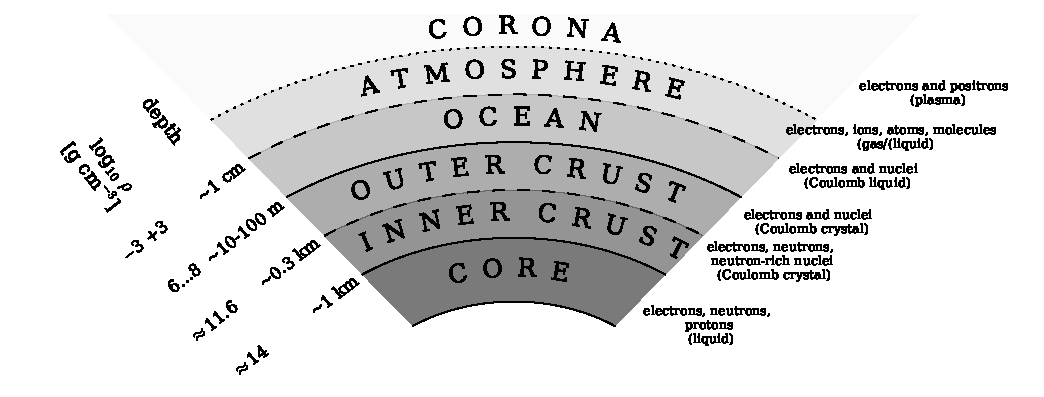
\includegraphics[width=13.5cm]{figs/slice/atmos.pdf}
\caption{\label{fig:pizza}
Schematic view of neutron star structure illustrating the different internal regions, related densities, and the compositions.
}
\end{figure}


\begin{figure}[t!]
\centering
\includegraphics[width=12.5cm]{figs/eos/eos.pdf}
\caption{\label{fig:eos}
Overview of the pressure versus density relation for the full range of densities relevant for neutron stars.
Here the evolution of the pressure is shown against the densities depicted in the bottom vertical axis.
Green solid line shows the EoS for matter at $T=10^6\Kelvin$, whereas blue line is for $T=\Ten{5}{6}\Kelvin$, and black for $T=10^7 \Kelvin$.
Additionally, the upper horizontal axis shows the evolution of the radial coordinate computed for one particular EoS (SLy, see \sect{sect:core}) and neutron star configuration (mass of $1.4\Msun$).
Different shaded vertical regions show the corresponding interior structures of the star.
Additionally, some interesting densities are highlighted with dashed red lines and text labels (see Sects.~\ref{sect:atmos}$-$\ref{sect:core}). 
}
\end{figure}

%sidewaysfigure

%\begin{sidewaysfigure}[t]
%\includegraphics[width=16cm]{figs/eos.pdf}
%\caption{\label{fig:eos}
%Overview of the pressure versus density relation for the full range of densities relevant for neutron stars.
%Here the evolution of the pressure is shown against the densities depicted in the bottom vertical axis.
%Green solid line shows the EoS for matter at $T=10^6\Kelvin$, whereas blue line is for $T=\Ten{5}{6}\Kelvin$, and black for $T=10^7 \Kelvin$.
%Additionally, the upper vertical axis shows the evolution of the radial coordinate computed for one particular EoS (SLy, see \sect{sect:core}) and neutron star configuration (mass of $1.4\Msun$).
%Different shaded vertical regions show the corresponding interior structures of the star.
%Additionally, some interesting densities are highlighted with dashed red lines and text labels (see Sects.~\ref{sect:atmos}$-$\ref{sect:core}). 
%}
%\end{sidewaysfigure}

In thermodynamics, we speak of \emph{state variables} that describe a current state of the matter under given physical conditions.
These include, for example, the density $\rho$, pressure $P$, and temperature $T$ of the matter.
Equation of state is a thermodynamical equation connecting these state variables together.
Often, when focusing on neutron stars, what we mean by EoS is a function connecting the pressure and the density of the matter only, $P(\rho)$.

The dependency on the rest of the variables such as temperature can be often forgotten because the matter is \emph{degenerate}. % \mnote{Degenerate matter}
In contrast to the ``normal'' matter where statistical moments such as temperature can be used to describe a large ensemble of particles, the degenerate matter is dominated by quantum mechanical effects of single particles.
Because of the immense densities, a free particle in degenerate matter is actually bounded into a finite volume.
Inside this small volume, the energy levels of the particle are restricted to take only a discrete set of values called quantum states, because of the underlying wave-nature of the quantum-mechanical description.
Hence, a notion of temperature, for example, does not make much sense.

An overview of the EoS for the full range of densities relevant to neutron stars is shown in \fig{fig:eos}.
From here it is easy to see that temperature only plays a role in the very uppermost $\osim 10\,\mathrm{meters}$ of the stars interiors.
Behavior of the matter is also quite well known all the way up to the crust-core interface, after which we start to see larger deviations because of the different EoS models.
In the laboratories on Earth, we can probe the matter somewhere close to $10^{14} \gcm$, after which the densities become too great for us to manipulate.%
\footnote{Maximum densities reached in the Earth are usually obtained by colliding heavy nucleons together, momentarily creating a core of even denser matter.
The densest naturally occurring element found on top of planet Earth is osmium that has an atomic density of ``just'' $\rho \approx \Ten{2.2}{1}\gcm$.
}
On the other hand, it is exactly starting from this density range that the bulk of the neutron star just starts.
Another curious quirk of Nature is how all of the complicated microphysics gets reduced to simple line segments in the logarithmic scales, also known as polytropic pressure relations.
In the following sections, we will focus on deriving these simple relations as it helps us in understanding the underlying physics.

\section{Atmosphere}\label{sect:atmos}
%Thin layer of plasma
%From centimeters in hot to millimeters in cold 
%Zavlin \& Pavlov 2002\cite{ZP02}
%\cite{Potekhin14}
%Where spectrum or thermal electromagnetic radiation is formed.
%Spectrum, beaming and polarization of emerging radiation can be determined from radiation transfer problem in atmospheric layers.
%thermal bb 
%magnetosphere powerlaw-like
%radiation espaces to the surrounding space without considerable losses.
%Gaseous uppermost layers.
%For strong magnetic field strenghts and low temperatures, the hydrogen can condensate into a liquid or solid surface.
%This is, however, quite rare and usually the hydrogen remains gaseous forming an atmosphere.

Atmosphere of a star is the first and uppermost layer responsible for the emergent radiation.
Usually, it consists of a thin layer of plasma and ranges from a few millimeters to a couple of centimeters in height, but in some cases if the emerging radiation field is strong enough it can momentarily expand the atmosphere up to several hundreds of meters.
%It consists of a thin layer of plasma and ranges from a few millimeters to couple of centimeters in height.
In most situations the plasma is in a gaseous state, but in some more rare cases when the magnetic field is extraordinarily strong and the temperature is low, the plasma can condense into a liquid or a solid surface.
Such condensed surfaces are, however, rare and usually the gaseous description is more than enough to give an accurate description of the physics of the atmosphere.\cite[see e.g.,][for a review]{ZP02, Potekhin14}

%Observationally we usually see either thermal radiation originating directly from the star's atmosphere, or a non-thermal power-law like component from the surrounding magnetosphere, or a combination of both.\cite[for a review, see][]{ZP02, Potekhin14}
%Properties of emergent radiation strongly depend on the chemical composition of the atmosphere.
%Difference to normal stars is that we only expect the composition to consist of the lightest element as heavier ones sink to the bottom.\cite{AI80}
%Consequence of gravitational force.

Properties of the emergent thermal radiation strongly depend on the chemical composition of the atmosphere.
In the atmospheres of normal stars, the composition is a mixture of multiple elements.
The most stable chemical element on the surface of a neutron star is iron.
However, even a small accreted mass of $10^{-17}\Msun$, originating from the surrounding interstellar medium or a binary companion, is enough to cover the whole star, and then a variety of elements are also expected in the neutron star atmospheres.
On the other hand, the enormous gravity results in an effective separation of elements leading to a strong sedimentation of the atmosphere where the lighter elements are expected to lay on top of the heavier ones, if the accretion does not constantly replenish the surface layers.\cite{AI80}
%Hence, the atmosphere is usually expected to consist of mainly hydrogen.


\subsection{General relativistic effects}
The effects from the gravity can be quantified by considering a so-called compactness parameter
\be
u = \frac{ R_{\mathrm{S}} }{R},
\ee
where $R$ is the radius of the neutron star and the corresponding Schwarzschild radius is defined as
\be
R_{\mathrm{S}} = \frac{2 G M}{c^2} \approx 2.95 \frac{M}{\Msun} \km,
\ee
where $G$ is the gravitational constant, $c$ is the speed of light, and $M$ is the mass of the star.\cite[see e.g.,][]{Gravitation, Wald84}
Hence, neutron star has a compactness parameter in the range of $u \approx 1/3$ to $1/2$ resulting in considerable general relativistic corrections.
In comparison, the Sun has $u \approx \Ten{4.24}{-6}$.
The compactness is also directly related to the gravitational redshift as
\be
1+z = (1-u)^{-1/2},
\ee
that describes how an energy of a photon changes when it has to climb up the gravitational potential well that is created by the star, for example.

Gravitational acceleration under general relativistic theory is
\be
g = \frac{G M}{R^2} \frac{1}{\sqrt{1-u}} = \Ten{1.38}{14} \frac{1}{\sqrt{1-u}} \left( \frac{M}{\Msun} \right) \left( \frac{10\km}{R} \right)^2 \cmss.
\ee
Hence, a surface gravitational acceleration $g$ of $\osim 10^{14}$ to $\osim 10^{15}\cmss$ is expected for neutron stars.
By considering an isothermal atmosphere we can also estimate the scale height as
\be
H_{\mathrm{a}} = \frac{k_{\mathrm{B}} T}{m_i g} \approx \frac{0.83}{A} \left( \frac{T}{10^6\Kelvin} \right) \left( \frac{10^{14} \cmss}{g} \right) \cm
\ee
where $k_{\mathrm{B}} = \Ten{1.38}{-16} \erg \unitspace \Kelvin^{-1}$ is the Boltzmann constant, $T$ is the temperature of the atmosphere, $m_i = A m_u$, and $m_u \approx \Ten{1.66}{-24}\g$ is the atomic mass unit.
From here, the typical scale height values of $\osim 1\cm$ to $\osim 10\cm$ are obtained for atmospheres of $T=10^6$ and $10^7\Kelvin$.\cite{ZP02, Potekhin14}
The strong gravitational field also bends the photon trajectories.\cite[see e.g.,][]{PFC83}
Hence, in addition to the radius $R$ of the star as measured in the local reference frame, another \emph{apparent} radius, as measured by an observer at infinity, 
\be
R_{\infty} = \frac{R}{\sqrt{1-u}},
\ee
is usually needed when describing the observable features of the atmosphere.
From here it is then clear that the atmosphere and the emerging radiation encodes information from the physical parameters of the star.
More specifically information about the temperature, surface gravity, chemical composition, and compactness can be obtained.

\subsection{Radiative transport in the atmosphere}
The standard approach in describing the atmosphere structure includes solving three main equations of radiative transfer, hydrostatic balance, and energy conservation.
First such a low-$B$ field model of hot neutron star atmospheres were presented in the pioneering work by London et al.\cite{London84,London86} and Lapidus et al.\cite{Lapidus85}.
Let us next walk through these equations, as they are rather simple.
A more general description for the atmosphere model computations are given in\cite{SPW12,NSK15}, where the fully relativistic electron scattering is also taken into account, whereas here we only consider the classical elastic (Thomson) scattering.

Because the thickness of the atmosphere is much smaller than the radius of the star,%
\footnote{Recall the scale height of $1$ to $10\cm$ in comparison to the radius of $10^6\cm$.}
the atmosphere can be considered in plane-parallel approximation.
Rather high densities, on the other hand, allow to consider the plasma of the atmosphere in local thermodynamical equilibrium.

Spectrum, beaming and polarization of emerging radiation can be determined from radiation transfer problem in atmospheric layers.
Radiation can be understood as an energy flow, i.e., energy $dE$ per area $dA$, time $dt$, frequency interval $d\nu$, and solid angle $d\Omega$.
This is known as the specific spectral intensity which we can mathematically formulate as
\be
I_{\nu} = \frac{dE}{dA \, dt \, d\nu \, d\Omega}.
\ee
Radiation averaged over the solid angle, or the so-called mean specific intensity (zeroth moment of $I_{\nu}$) is then
\be
J_{\nu} = \frac{1}{4\pi} \int_{\Omega} I_{\nu} d\Omega 
= \frac{1}{4\pi} \int_0^{2\pi} d\phi \int_0^{\pi} I_{\nu} \sin\theta d\theta = \frac{1}{2} \int_{-1}^{+1} I_{\nu} d\mu,
\ee
where we have assumed that the radiation does not depend on the azimuthal $\phi$ angle (as is typical for atmosphere calculations) and introduced $\mu \equiv \cos\theta$ as the cosine of the zenith angle.
Net rate of energy flowing across a unit area (for example a photon detector) from \emph{all directions} per time and frequency is known as physical flux.%
\footnote{
    Strictly speaking, the first-order moment of $I_{\nu}$ is known as the Eddington flux $H_{\nu} = \frac{1}{2} \int_{-1}^{+1} I_{\nu}\mu d\mu$.
    Physical flux is related to it as $F_{\nu} = 4\pi H_{\nu}$ and sometimes one also encounters the ``astrophysical'' flux defined as $F_{\nu}/\pi$.
}
It is proportional to the first-order moment of $I_{\nu}$ and is defined as
\be
F_{\nu} = 2\pi \int_{-1}^{+1} I_{\nu} \mu d\mu.
\ee
Similarly, the second-order moment of $I_{\nu}$, or a so-called K-integral, is
\be
K_{\nu} = \frac{1}{2} \int_{-1}^{+1} I_{\nu} \mu^2 d\mu,
\ee
which is related to the radiation pressure, as we later on will see.

Now we can introduce the radiative transfer equation for $I_{\nu}$ as
\be\label{eq:rte}
\mu \frac{d I_{\nu}}{d\tau} = \frac{\mu}{\kappa_{\nu}} \frac{d I_{\nu} }{dy} = -\frac{\mu}{\rho \kappa_{\nu}} \frac{d I_{\nu} }{dz } = I_{\nu} - S_{\nu}
\ee
where $\tau$ is the optical depth, $y$ is the column density (mass per area), $z$ is the vertical distance from the surface, $\kappa_{\nu} = \alpha_{\nu} + \sigma_{\nu}$ is the total radiative opacity including contributions from the ``true'' opacity $\alpha_{\nu}$ and from the scattering opacity $\sigma_{\nu}$.
Here the connection between different independent variables is given as
\be
d\tau = \kappa_{\nu} dy = -\kappa_{\nu} \rho dz,
\ee
relating the optical depth (distance as experienced by the radiation), column density (projected number density of matter along the path of the radiation), and the height.
In addition, we need the source function 
\be
S_{\nu} = (\sigma_{\nu} J_{\nu} + \alpha B_{\nu}) \kappa_{\nu}^{-1},
\ee
where the scattering term is proportional to the mean spectral intensity $J_{\nu}$ and the ``true'' absorption term to the thermal Planck function
\be
B_{\nu}(T) = \frac{2 h \nu^3}{c^2} \frac{1}{\exp \left[ h \nu/(k_{\mathrm{B}}T) \right] -1 },
\ee
where $h = \Ten{6.63}{-27} \unitspace \erg \unitspace \mathrm{s}$ is the Planck constant.
As a boundary condition for this equation, we can use $I_{\nu} = 0$ for $\mu < 0$ at $y = 0$ (i.e., the surface).
The atmospheres are also usually considered to be in radiative and hydrostatic equilibrium, i.e., (quasi-)stationary.
The first requirement assumes that energy is transported by radiation only, i.e., we neglect, for example, conduction and convection.
The energy balance in the atmosphere can then be expressed via the radiation flux $F$ only as 
%The first requirement can be expressed via the effective temperature $T_{\mathrm{eff}}$ as 
\be
\int_0^{\infty} d\nu \int_0^{2\pi} d\phi  \int_{-1}^{+1} I_{\nu} \mu d\mu = F = \sigma_{\mathrm{SB}} T_{\mathrm{eff}}^4,
\ee
where $\sigma_{\mathrm{SB}} = \Ten{5.67}{-5} \unitspace \erg \unitspace \mathrm{cm}^{-2} \unitspace \mathrm{s}^{-1} \unitspace \Kelvin^{-4}$ is the Stefan-Boltzmann constant, and $T_{\mathrm{eff}}$ is the effective temperature.
%where $\sigma_{\mathrm{SB}} = \Ten{5.67}{-5} \unitspace \g \unitspace \mathrm{s}^{-3} \unitspace \Kelvin^{-4}$ is the Stefan-Boltzmann constant \blue{I prefer erg/cm2/s/K4 as it shows that it relates temperature to the flux} and $T_{\mathrm{eff}}$ is the effective temperature of the atmosphere.
The second requirement of hydrostatic equilibrium, demands that
\be
\frac{dP_{\!\mathrm{g}}}{dy} = g - g_{\mathrm{rad}},
\ee
where, in addition to the gravitational acceleration $g$ we need the opposing radiative acceleration $g_{\mathrm{rad}}$.
Finally, we need to supplement these equations with an equation connecting the gas pressure $P_{\!\mathrm{g}}$ and density.
For the rarefied atmosphere, the ideal gas law is an excellent approximation
\be\label{eq:idealgaslaw}
P_{\!\mathrm{g}} = n k_{\mathrm{B}} T,
\ee
where $n$ is the number density of particles.

\subsection{Eddington limit}\label{sect:Eddington}
Usually the atmospheres we calculate are dynamically stable and in hydrostatic balance because large gravity implies $g_{\mathrm{rad}} \ll g$.
Sometimes, however, the radiation flux might increase to such a strength that it is able to compete against even the enormous gravity of a neutron star.
An important limit can then be defined for $g_{\mathrm{rad}} = g$, known as the Eddington limit after a renowned astrophysicist Sir Arthur Eddington.
Let us now for completeness derive this limit.\cite[see e.g.,][]{RL79, FKR02}

We can start by formulating an expression for the radiation pressure.
This can be easily done when we realize that pressure is just flow of momentum through a surface per unit time and photons carry a momentum of $E/c = h\nu/c$, i.e., projection of the radiation flux into the surface that is considered.
%\footnote{
%    Energy of a photon is $E=h\nu=mc^2$, from which we obtain the photon rest mass of $h\nu/c^2 = E/c^2$. 
%    Momentum, on the other hand, is just velocity times the mass, so for a photon it is $E/c^2 \times c = E/c$.
%}
In terms of $I_{\nu}$ this is then
\be
P_{\mathrm{rad}, \nu} = \frac{1}{c} \int_0^{2\pi} d\phi \int_{-1}^{+1} I_{\nu} \mu^2 d\mu = \frac{4\pi}{c} K_{\nu},
\ee
relating the pressure and the second-order moment $K_{\nu}$ together.
Radiative acceleration is then
\be\label{eq:grad}
g_{\mathrm{rad}} = \frac{d P_{\mathrm{rad}}}{dy} = \frac{d}{dy} \int_0^{\infty} P_{\mathrm{rad},\nu} \, d\nu = \frac{4\pi}{c} \frac{d}{dy} \int_0^{\infty} K_{\nu} d\nu.
\ee
Let us refine this expression by inserting the definition of $K_{\nu}$ and applying the radiative transfer equation \eq{eq:rte} in the subsequent equation to obtain
\begin{align}\begin{split}\label{eq:kfgradnu}
    g_{\mathrm{rad}} &= \frac{4\pi}{c} \frac{d}{dy} \int_{0}^{\infty} d\nu \frac{1}{2} \int_{-1}^{+1} I_{\nu} ~ \mu^2 d\mu \\
                     &= \frac{2\pi}{c} \int_0^{\infty} d\nu \int_{-1}^{+1} \mu \, d\mu ~ \left\{ \mu \frac{d}{dy} I_{\nu} \right\}  \\
                     &= \frac{2\pi}{c} \int_0^{\infty} d\nu \int_{-1}^{+1} \mu \, d\mu ~  \left\{ \kappa_{\nu} I_{\nu} - \kappa_{\nu} S_{\nu} \right\}.
\end{split}\end{align}
We can then simplify equation \eq{eq:kfgradnu} further by assuming isotropic source function $S_{\nu}(\mu) = S_{\nu}$ and opacity $\kappa_{\nu}(\mu) = \kappa_{\nu}$ to get
\begin{align}\begin{split}\label{eq:kfgrad}
    g_{\mathrm{rad}}
                     &= \frac{2\pi}{c} \int_0^{\infty} d\nu \int_{-1}^{+1} \mu \, d\mu ~  \kappa_{\nu} I_{\nu} 
                       - \frac{2\pi}{c} \int_0^{\infty} d\nu \int_{-1}^{+1} \mu \, d\mu ~  \kappa_{\nu} S_{\nu}\\
                     &= \frac{2\pi}{c} \int_0^{\infty} d\nu ~\kappa_{\nu} \int_{-1}^{+1} I_{\nu} \mu d\mu + 0\\
                     &= \frac{1}{c} \int_0^{\infty} ~ \kappa_{\nu} F_{\nu} d\nu \\
                     &= \frac{1}{c} \kappa_{\mathrm{F}} F,
\end{split}\end{align}
where $F = \int_0^{\infty}F_{\nu} d\nu$ is the bolometric flux, and 
\be
\kappa_{\mathrm{F}} = \frac{1}{F} \int_0^{\infty} \kappa_{\nu} F_{\nu} d\nu,
\ee
is the flux mean opacity.\cite{MM84,Poutanen17}
%\be
%\int_{-1}^{+1} \kappa_{\nu} S_{\nu} ~\mu d\mu = \int_{0}^{+1} ( \sigma_{\nu} J_{\nu} + \alpha_{\nu} B_{\nu} ) \mu d \mu = 0 + 0,
%\ee
%because both $J_{\nu}$ and $B_{\nu}$ are isotropic, i.e. do not depend on the angles.
From Eq. \eqref{eq:kfgrad} we then see that the radiation acceleration is directly related to the flux of the radiation.
Not every photon, however, interacts and collides with the matter, and hence the opacity correction $\kappa_{\mathrm{F}}$ is also needed. %, representing effectively the fraction of radiation interacting with the matter.
%If we now integrate over all the frequencies we obtain
%\be
%g_{\mathrm{rad}} = \frac{1}{c} \kappa F
%\ee
Setting \eqref{eq:kfgrad} equal to $g$ we can solve for the Eddington flux as
\be
F_{\mathrm{Edd}} = \frac{g c }{\kappa_{\mathrm{F}}} = \frac{G M c}{R^2 \kappa_{\mathrm{F}}} \frac{1}{\sqrt{1-u}}.
\ee
Usually in many astrophysical scenarios the opacity is dominated by the electron scattering opacity with a characteristic (Thomson) cross-section for the interaction $\sigma_{\mathrm{T}} = \Ten{6.65}{-25} \unitspace \mathrm{cm}^{-2}$.
Mass for a hydrogen plasma, on the other hand, is mainly set by the protons, hence, opacity per unit mass is then
\be
\kappa_{\mathrm{F}} \approx \frac{ \sigma_{\mathrm{T}} }{m_{\mathrm{p}}} \approx 0.4 \cm^2\unitspace\g^{-1}.
\ee
Finally, by calculating the total radiation flux through the stellar surface, we can define a quantity called luminosity as
\be
L = 4\pi R^2 F(R),
\ee
where $F(R)$ is the outcoming radiation flux at the surface.
Using the aforementioned equation, we can then define the Eddington luminosity for a star as 
\be\label{eq:Ledd}
L_{\mathrm{Edd}} = \frac{4\pi G M c m_{\mathrm{p}} }{\sigma_{\mathrm{T}} } \approx \Ten{1.3}{38} \left( \frac{M}{\Msun} \right) \ergs.
\ee
For neutron stars with surface temperature of $T \sim 10^7 \Kelvin$ this limit can be reached, after which the atmosphere can momentarily expand to counter the excess force as exerted by the radiation.



%\subsection{Radiative heat transfer}
%Let us also shortly characterize the time-dependency of the energy transfer in the atmosphere.\cite[for a more in depth discussion, see][]{CM04, iZCT14}
%Such an analysis will also be observationally important because in some cases we do see short bursts of energy coming from the neutron stars, called X-ray bursts.\cite[for a review, see e.g.,][]{LvPT93, GMH08}

%If we deposit an energy $Q$ into somewhere deep below the atmosphere, this energy will be transferred to the surface, and then freely radiated to us.
%In general, this heat energy is
%\be
%Q = m C_P T,
%\ee
%where $m$ is the mass of the cooling layer, $C_P$ is the specific heat capacity at a constant pressure, and $T$ is the temperature of the layer.
%Assuming, as a first approximation, constant opacity for the atmosphere, the heat is transferred simply according to Stefan-Boltzmann law as
%\be
%\frac{dQ}{dt} =  -A \sigma_{\mathrm{SB}} \frac{ T^4}{\tau} = -A \sigma_{\mathrm{SB}} T_{\mathrm{eff}}^4 ,
%\ee
%where $t$ is now the time, $A$ is the area that the heat radiation propagates through, $T_{\mathrm{eff}}$ is the effective temperature of the atmosphere, and $\tau$ is the optical depth, as given before.
%Temperature solved from this is simply
%\be
%T_{\mathrm{eff}} =\left( \frac{3 A \sigma_{\mathrm{SB}} }{m C_P } t \right)^{-1/3}.
%\ee
%Assuming all of the energy goes into radiation, we then obtain
%\be
%L = -\frac{dQ}{dt} = A \sigma_{\mathrm{SB}} T_{\mathrm{eff}}^4 
%  = (A \sigma_{\mathrm{SB}} )^{-1/3} \left( \frac{3}{m C_P} t \right)^{-4/3}.
%\ee
%Hence, energy deposited below the atmosphere will radiate to us and decay as $\propto t^{-4/3}$.
%In general, the heat capacity is $C_P = C_P(T)$, but the main results hold, that observationally we should see a powerlaw decay of luminosity, if an excess energy is instantaneously injected or released into the deeper layers of the star. 



\section{Crust}
%Outer crust
%From atmosphere to $\rho_{\mathrm{ND}} \sim \Ten{4}{11} \gcm$.
%In thickness some hundred meters.
%Non degenerate electron gas.
%Ultra-relativistic electron gas $\rho > 10^6 \gcm$.
%Pressure provided by electrons here.
%In deeper layers ions form a strongly coupled Coulomb system (liquid or solid).
%Hence, crust.
%At the base neutrons start to drip out from nuclei.

Below the gaseous atmosphere, a solidified layer of matter exists, called crust.\cite[see e.g.,][for a review]{HPY07, CH08, NSCrust12}
Between the atmosphere and crust, a liquid ocean of ions also exists, but the interface is not very strict and the matter is smoothly evolving from one state to another.
The solidified crust is also typically divided into an outer and inner layer, but the interface is again ambiguous. 
The pressure here is dominated by the degenerate electrons. 
In the beginning, the electrons can be taken to be non-relativistic but at about $\rho \!\sim\! 10^{6} \gcm$ they turn ultra-relativistic because of the increasing density.

By definition, the outer crust is a layer in the neutron star interior where the plasma consists of electrons and nuclei, whereas the inner crust is characterized by an additional appearance of neutrons that start to drip out from the extremely neutron-rich nuclei.
The density this occurs is called the neutron drip density and is around $\rho_{\mathrm{ND}} \sim \Ten{4}{11} \gcm$.
The outer crust, when defined to begin from the atmosphere at $\rho \sim 10^3 \gcm$ and continue to about $\rho_{\mathrm{ND}}$ is only about some hundred meters thick.
The characteristics of the matter are strongly dependent on the Coulomb interactions of charged particles that form a solid Coulomb crystal.

%\subsection{Inner crust}
%About one kilometer thick.
%Density from $\rho \sim \rho_{\mathrm{ND}}$ (at upper boundary) to $\sim 0.5 \nsat$ at the base.
%Matter consists of electrons, free neutrons $n$ and neutron-rich atomic nuclei.
%Fraction of free $n$ grow with $\rho$.
%
%nuclei are immersed in a neutron gas and hence nuclear interactions play a crucial role in defining the matter.
%Finally, nuclei disappear at the crust-core interface.

The inner crust is taken to continue all the way down to the crust-core interface, where the matter turns liquid again.
This layer is about one kilometer thick.
Here, at the bottom of the crust, the density is already close to the nuclear density of $\rho_{\mathrm{n}} = \Ten{2.8}{14} \gcm$ but the exact location of the transition depends on the detailed microphysics of the core.
The fraction of free neutrons grows with the increasing density.
Because the normal nuclei here are immersed into free neutron gas, the nuclear interactions play a crucial role in defining the matter.
Finally, the nuclei disappear totally when we enter the core.
Before that, however, the nuclei form complicated structures that evolve together with the density.
This region is also known as the nuclear pasta phase, as the different structures are named after the pasta types that they resemble.\cite[see e.g.,][]{CH16}


\subsection{Fermi gases}
The matter in the crust is degenerate.\cite[see e.g.,][]{LL80}
Let us discuss the physics behind degenerate matter and the related important concept of Fermi energy now.
Elementary 6-dimensional phase space cell of any particle is bounded by the Heisenberg uncertainty principle as
\be\label{eq:pcell}
\Delta x \Delta y \Delta z \Delta p_{x} \Delta p_{y} \Delta p_{z} = h^3,
\ee
where $\Delta x\Delta y \Delta z$ is the volume in ordinary space, $\Delta p_x \Delta p_y \Delta p_z$ the volume in the momentum space, and $h$ is the previously defined Planck constant.
In general the number density is given as
\be\label{eq:dist}
n_{\mathrm{av}} = \frac{g}{\exp[ (E-\mu)/k_{\mathrm{B}}T ] \pm 1},
\ee
where $+$ is used for fermions (such as electrons and protons), and $-$ for bosons (such as photons).
Additionally, the $g$ is the number of different quantum states a particle may have inside the cell, $E$ is the total particle energy, and $\mu$ is the chemical potential that describes the free energy content of the system per particle. %explained more carefully later on.
%\refedel{In} \refedel{accordance} \refedel{with} \refedel{the} \refedel{quantum} \refedel{mechanics,} \refedel{there} \refedel{is} \refedel{room} \refedel{for} \refedel{only} \refedel{one} \refedel{fermion} \refedel{inside} \refedel{the} \refedel{elementary} \refedel{cell}.
%%\footnote{Note that the chemical potential $\mu$ defined here should not be mixed with the cosine of the normal angle, as defined in the previous section when dealing with atmospheres.
%The difference should be clear from the context so same variable name is used here.}
Number of particles per unit volume with momentum between $p$ and $p+dp$ is 
\be\label{eq:pshell}
n(p) dp = n_{\mathrm{av}} \frac{4\pi p^2}{h^3} dp,
\ee
i.e., particles inside a spherical shell with a surface $4\pi p^2$ and thickness $dp$.
Number density of particles with all momenta is then
\be
n = \int_0^{\infty} n(p) dp.
\ee
%and the density is then simply
%\be
%\rho = n m,
%\ee
%where $m$ is the mass of the particle.
The energy in equation \eq{eq:dist} is the total energy $E \equiv E_{\mathrm{tot}} = E_0 + E_{\mathrm{k}}$, composed of the rest-mass energy $E_0 = mc^2$ and kinetic energy $E_{\mathrm{k}}$.
In special relativity, there exists a relation for the total energy as $E_{\mathrm{tot}}^2 = (mc^2)^2 + (pc)^2$, so 
\be\label{eq:totener}
E = mc^2 \left[ 1 + \left(\frac{p}{mc} \right)^2 \right]^{1/2},
\ee
and the kinetic energy is then simply
\be
E_{\mathrm{k}} = mc^2 \left[ \left( 1 + \left(\frac{p}{mc} \right)^2 \right)^{1/2} - 1 \right].
\ee
Simple asymptotic limits can be obtained for the kinetic energy as
\be\label{eq:asymplims}
E_{\mathrm{k}} \approx
\begin{cases}
      ~\displaystyle\frac{p^2}{2m} \quad & \text{if } p \ll mc ~  \text{(non-relativistic)} \\
      ~pc \quad & \text{if } p \gg mc ~ \text{(ultra-relativistic)}. \\
      \end{cases}
\ee

Let us now focus on fermions only and select the $+$-sign (Fermi-Dirac distribution) in Eq. \eqref{eq:dist}.
Fermions are characterized as spin-$\frac{1}{2}$ particles.
In accordance with the quantum mechanics, there is room for only one fermion inside an elementary cell \eqref{eq:pcell}.
The degeneracy parameter $g$ is then equal to $2$ because we can have particles of spin $-\frac{1}{2}$ and $+\frac{1}{2}$ in the same ``physical location'' ($\Delta x \Delta y \Delta z$), as they still have different ``momentum locations'' ($\Delta p_x \Delta p_y \Delta p_z$) in phase space because of the non-equal spins.

The chemical potential $\mu$ in Eq. \eqref{eq:dist} can be expressed as
\be
\mu = \ef +  (E -  E_{\mathrm{k}}),
\ee
where $\ef$ is a reference energy level known as the Fermi energy.
This reflects how the chemical potential is equal to the amount of energy that can be liberated from the system. 
This is also known as chemical energy.
%On the other hand, the chemical potential can also be written as
%\be
%E - \mu = E_{\mathrm{k}} - \ef
%\ee
%i.e., difference between the kinetic and Fermi energy.
Hence, the number density of fermions in general is
\be\label{eq:FD}
n_{\mathrm{f}}= \frac{8 \pi}{h^3} \int_0^{\infty} \frac{p^2 dp}{ \exp ( \frac{ E_{\mathrm{k}} - \ef }{ k_{\mathrm{B}} T } ) + 1}.
\ee
If the Fermi energy $\ef \ll k_{\mathrm{B}} T$, the distribution will be Maxwellian even for small kinetic energies.
On the other hand, if $\ef \gg k_{\mathrm{B}}T$ we can divide the integrand of Eq. \eqref{eq:FD} into two distinct regions of 
\be
\frac{p^2}{ \exp ( \frac{ E_{\mathrm{k}} - \ef }{ k_{\mathrm{B}} T } ) + 1} \approx 
\begin{cases}
    ~p^2 \quad &\text{if } E_{\mathrm{k}} \ll \ef \\
    ~0 \quad   &\text{if } E_{\mathrm{k}} \gg \ef, \\
\end{cases}
\ee
with a sharp transition in between at $E_{\mathrm{k}} \approx \ef$.
This allows us to define a characteristic momentum related to the transition energy $\ef$, called Fermi momentum $p_{\mathrm{F}}$, so that
\be
n_{\mathrm{f}} \approx \frac{8\pi}{h^3} \int_0^{p_{\mathrm{F}}} p^2 dp = \frac{8\pi}{3} \left( \frac{p_{\mathrm{F}}}{h} \right)^3.
\ee
Physically this can be interpreted such that when the temperature decreases, the fermions start to occupy all the quantum states starting from the one with the lowest energy all the way up to the Fermi energy.
Because of the Pauli exclusion principle, no more than one fermion can exist in the same quantum state so the levels are filled in order, and all the higher states will remain empty.
Hence, the highest momenta possible in the fully degenerate matter is the Fermi momentum given as 
\be\label{eq:fermimom}
p_{\mathrm{F}} = \left( \frac{3 n_{\mathrm{f}}}{8 \pi} \right)^{1/3} h.
\ee
It is, of course, also related to the Fermi energy simply as
\be
\ef = \frac{1}{2} \frac{ p_{\mathrm{F}}^2 }{ m },
\ee
that we previously defined merely as a reference energy level.
However, from this, the physical interpretation should also become clear as Fermi energy corresponds to the energy of the highest quantum state occupied in the system when temperature reaches zero.



\subsection{Why neutrons then?}
%Fermi energy grows with increasing $\rho$.
%Induces $\beta$ captures and enriches nuclei with neutrons.
%Fermi energy is also an important concept that can be used to describe the physics of the matter.
%\red{define Fermi energy}
%This Fermi energy increases with increasing $\rho$.
%This, in turn, induces $\beta$ captures and enriches nuclei with neutrons.

Let us first consider an ideal gas of degenerate electron-proton-neutron plasma to understand the basic composition of the crust.\cite[see e.g.,][]{Phillips94}
In a degenerate plasma all the quantum states are filled up all the way to the Fermi energy, as we just learned.
The normal beta-decay mode for the neutrons, on the other hand, is 
\be
n \rightarrow p + e^{-} + \bar{\nu_{e}},
\ee
that describes the possible path of how a neutron $n$ will decay into a proton $p$, electron $e^{-}$, and electron antineutrino $\bar{\nu_{e}}$.
It is because of this decay, that we do not expect to see any free neutrons flying around.
Such a natural decay, however, might be blocked because there is no room for an emission of an extra electron $e^{-}$ or a proton $p$.

Let us then only focus on the decay of the most energetic neutrons with an energy equal to the Fermi energy $\ef(n)$, where the related particle species is now defined inside the parentheses for clarity.
Co-existence of neutrons, protons, and electrons is guaranteed (at zero temperature) if 
\be
\ef(n) = \ef(p) + \ef(e^{-}).
\ee
%Fermi momentum of a particle is related to its concentration via
%\be
%p_{\mathrm{F}} = \left( \frac{3n}{8\pi} \right)^{1/3} h,
%\ee
%where $n$ is the number density, and $h$ the Planck constant.
Massive neutrons and protons are to a good approximation non-relativistic up to densities of $10^{14}\gcm$, and hence energy is simply a sum of their rest mass energy and kinetic energy
\be
\ef(n) \approx m_n c^2 + \frac{p_{\mathrm{F}}(n)^2}{2 m_n },
\ee
and
\be
\ef(p) \approx m_p c^2 + \frac{p_{\mathrm{F}}(p)^2}{2 m_p }.
\ee
Electrons, on the other hand, are already ultra-relativistic, and so
\be
\ef(e^{-}) \approx p_{\mathrm{F}}(e^{-}) c.
\ee
Also note that $n_p = n_e$, as the star is electrically neutral.

From this we can solve $n_n/n_p \sim 5$, $100$, and $1000$ for $\rho \sim 10^8$, $10^9$, and $10^{10} \gcm$, respectively, by taking into account the rest mass difference $m_n - m_p \approx 1.3 \unitspace\mathrm{MeV}\unitspace c^2$.
Thus, we conclude that the matter inside is expected to be neutron rich, even though normally the neutrons would $\beta$-decay back to protons and electrons.
Not only is the degeneracy then responsible for the pressure but it is also the source of the neutron enrichment. 


\subsection{Degenerate electron gas}
Let us next consider the equation of state for the crust.
As we have seen, the pressure in the crust originates from the degenerate electron gas.
The physics behind this are quite simple, and we repeat the calculations here to introduce the reader to the topic.
The result also bears some historical value as these are the equations that were first introduced by Dirac\cite{Dirac25}, Fowler\cite{Fowler26}, Frenkel\cite{Frenkel28}, Anderson\cite{Anderson29}, Stoner\cite{Stoner30}, and Chandrasekhar\cite{Cha31}.\cite[see also][]{Cha39, Schatzman58, Salpeter61, Tooper69, ZN71, LL80, Blinnikov87, YS89, HPY07}
%\cite[For a review, see e.g.,][]{Cha39, LL80, HPY07}

The behavior of the matter in the crust is dominated mainly by the electrons. 
For this reason, it can be characterized by the electron number density $n_{\mathrm{e}}$ and temperature $T_{\mathrm{e}}$, hereafter just $T$ in this section.
Instead of $n_{\mathrm{e}}$, let us use the electron Fermi momentum $p_{\mathrm{F}}$ \eq{eq:fermimom} as a measure of the number density.
It is convenient to describe it in the units of electron rest mass, as
\be
\xr \equiv \frac{p_{\mathrm{F}}}{\me c},
\ee
also known as the relativity parameter.\cite{Salpeter61}
We will also need the more generic special relativistic form of the Fermi energy
\be
\epsilon_{\mathrm{F}} = c \sqrt{ ( \me c)^2 + p_{\mathrm{F}}^2 },
\ee
that for a strongly degenerate gas, has the meaning of the chemical potential $\mu$.
Finally, the electron Fermi temperature is
\be
T_{\mathrm{F}} = \frac{\me c^2}{k_{\mathrm{B}}} \left( \sqrt{1 + \left( \frac{ p_{\mathrm{F}} }{\me c } \right)^2 } - 1 \right)
= \Tr ( \gammar -1 ),
\ee
where a typical temperature is
\be
\Tr = \frac{ \me c^2 }{k_{\mathrm{B}}} \sim \Ten{6}{9} \Kelvin,
\ee
and a relativistic scaling factor is defined as
\be
\gammar \equiv \sqrt{1 + \xr^2}.
\ee
Then, the temperature can also be expressed in units of $T_{\mathrm{r}}$ as 
\be
t_{\mathrm{r}} \equiv \frac{T}{\Tr}.
\ee
Using these definitions, it is easy to characterize how relativistic the electron gas is.
We can divide it into three regions of 
\begin{itemize}
    \item non-relativistic, for which $t_{\mathrm{r}} \ll 1 $ and/or $\xr \ll 1$, 
    \item mildly-relativistic, $t_{\mathrm{r}} \sim 1$ and/or $\xr \sim 1$,
    \item ultra-relativistic, $t_{\mathrm{r}} \gg 1$ and/or $\xr \gg 1$.
\end{itemize}

Similarly, we can scale the temperature with the Fermi temperature to get a so-called degeneracy parameter
\be\label{eq:Thetar}
\Theta_{\mathrm{F}} \equiv \frac{T}{T_{\mathrm{F}}}.
\ee
It can be then used to characterize the degeneracy of the plasma to regions of 
\begin{itemize}
    \item non-degenerate, for which $\Theta_{\mathrm{F}} \gg 1$,
    \item mildly degenerate, $\Theta_{\mathrm{F}} \sim 1$,
    \item and strongly degenerate, $\Theta_{\mathrm{F}} \ll 1$.
\end{itemize}


Moving on from an ideal gaseous plasma in the atmosphere, we can start by introducing corrections produced by the closely packed charged particles.
In practice, we use the so-called ion-sphere model to describe our Coulomb liquid of ions.
We now assume that our ions are emerged into a sea of rigid electron background that takes care of the charge neutrality.
In order to couple the number density of electrons and the mass of the plasma, let us first define the mean charge per mass ratio of the plasma as
\be
\Mu = \frac{\bra{Z}}{\bra{A}},
\ee
where $\bra{Z}$ is the mean charge number of the atomic nuclei (for a one-component plasma it is simply $Z$), and $\bra{A}$ is the average number of nucleons bound by one nucleus.
For most plasmas, $\Mu \approx \frac{1}{2}$.

Let us now begin by defining a so-called electron sphere radius as
\be
\erad = \left( \frac{4\pi \nel}{3} \right)^{-1/3}.
\ee
We can also parameterize the strength between Coulomb (charge) interactions by considering a ratio of potential energy to the kinetic energy with
\be
\Ge = \frac{e^2}{\erad k_{\mathrm{B}} T} \approx 22.75 \left( \frac{10^6 \Kelvin}{T} \right) \left( \frac{\rho}{10^6 \gcm} \right)^{1/3} \Mu^{1/3},
\ee
where $e = \Ten{4.80}{-10} \unitspace \mathrm{esu}$ is the electron charge.
Similarly, for ion with a charge number of $\Zi$, we can define the ion-sphere radius
\be
\irad = \erad \Zi^{1/3},
\ee
that encapsulates enough volume to be charge neutral, when considering the static electron-induced background from $\nel$.
Ion Coulomb coupling factor is similarly
\be
\Gi = \Ge \Zi^{5/3} = \frac{ (\Zi e)^2}{\irad k_{\mathrm{B}} T}.
\ee

At high temperatures, the electrons form a classical Boltzmann gas.
When the temperature is decreased, the plasma will then become a strongly coupled Coulomb liquid corresponding to the neutron star ocean.
If the temperature is decreased further, the plasma will transform into a Coulomb crystal. % with a phase transition.
The gaseous regime can be constrained to be at $\Gi \ll 1$, or $T \gg T_{\mathrm{B}}$, where the $T_{\mathrm{B}}$ is given as
\be
T_{\mathrm{B}} = \frac{Z^2 e^2}{a_i k_{\mathrm{B}}} \approx \Ten{2.28}{7} \left( \frac{\rho}{10^6 \gcm} \right)^{1/3} \Mu^{1/3} \Kelvin.
\ee

The pressure for such a system can be obtained via the standard thermodynamical relation
\be\label{eq:press}
P = \left( \frac{\partial F}{\partial V} \right)_{T},
\ee
where $F$ is the Helmholtz free energy and $V$ is the volume of the system.\cite[see e.g.,][]{LL80}
It is useful to divide the free energy into an ideal part $F_{\mathrm{id}}$ corresponding to non-interacting particles, and to the excess part $F_{\mathrm{ex}}$, leading to 
\be
F(V, T) = F_{\mathrm{id}} + F_{\mathrm{ex}}.
\ee
Similarly, we could decompose the ideal effects from ions to $F_{\mathrm{id}}^{(\mathrm{i})}$ and from electrons to $F_{\mathrm{id}}^{(\mathrm{e})}$, yielding
\be
F(V, T) = F_{\mathrm{id}}^{(\mathrm{i})} + F_{\mathrm{id}}^{(\mathrm{e})} + F_{\mathrm{ex}}.
\ee
Most important non-ideal deviation for the plasma is from the Coulomb interaction between ions and electrons, and between electrons in the rigid background $F_{\mathrm{ex}} \approx F_{\mathrm{ii}}$.
This free energy decomposition then induces similar division for the pressure
\be
P \approx P_{\mathrm{id}}^{(\mathrm{i})} + P_{\mathrm{id}}^{(\mathrm{e})} +  P_{\mathrm{ii}}.
\ee

The main contributor for the pressure is the electron degeneracy pressure, $P_{\mathrm{id}}^{(\mathrm{e})}$.
Other terms, given as $|P_{\mathrm{part}}|/P_{\mathrm{id}}^{(\mathrm{e})}$, result in leading order terms of\cite{YS89} 
\be\label{eq:pressvalidity}
\frac{P_{\mathrm{id}}^{(\mathrm{i})} }{ P_{\mathrm{id}}^{(\mathrm{e})} } \approx \frac{ \Theta_{\mathrm{r}}^{(\mathrm{i})} }{Z}
\ee
\be
\frac{P_{\mathrm{ii}} }{P_{\mathrm{id}}^{(\mathrm{e})}} \approx \alpha_{\mathrm{f}} \frac{ \gammar }{ x_{\mathrm{r}} },
\ee
where $\Theta_{\mathrm{r}}^{(\mathrm{i})}$ is the temperature in units of nucleon Fermi temperature (see Eq. \ref{eq:Thetar}), $\alpha_{\mathrm{f}} = e^2 /\hbar c \approx 1/137$ is the fine-structure constant, and $\hbar = h/2\pi$.
From here it is easy to see that only the Coulomb interaction term $P_{\mathrm{ii}}$, should give a measurable correction to the pressure at low temperatures because for the conditions inside neutron stars $\Theta_{\mathrm{r}}^{(\mathrm{i})}$ is very small.
This suggests that for the pressure $P$ we can use the approximation
\be\label{eq:approxpress}
P \approx P_{\mathrm{id}}^{(\mathrm{e})} + P_{\mathrm{ii}}.
\ee

In the weak-coupling limit ($\Gi \ll 1$) the Debye-H\"uckel result for the excess free energy is a sufficiently good approximation, expressed as\cite{DH23, LL80, ST83, DeWitt96}%
\footnote{Debye-H\"uckel approximation relays on the assumption that the charge density surrounding an ion is described by electrostatics (Poisson's equation) and the distribution of the charge around the ion itself by thermal motions of electrons (Boltzmann's equation).
}
\be
\frac{F_{\mathrm{ex}}}{V} = \frac{1}{\sqrt{3}} n_{\mathrm{i}} kT \Gi^{3/2},
\ee
where $n_{\mathrm{i}}$ is the ion number density.
Hence, the pressure correction due to the Coulomb interactions can be simply presented as 
\be
\Pii \approx -0.3 n_{\mathrm{i}} \frac{Z^2 e^2}{\irad}
\ee
by using Eq. \eq{eq:press}.
Note also that $\Gi = \Gi(V)$ when taking the derivative in respect to the volume when deriving the expression for the pressure.

Let us, as a final task, look into the main degenerate electron pressure term $P_{\mathrm{id}}^{(\mathrm{e})}$.
Pressure is defined as a flux of momentum through a surface, hence for one particular wall it is
\be\label{eq:vpress}
P = \int_0^{\infty} \bra{v_x p_x} n(p) dp,
\ee
where the number density $n(p)$ is desribed by the Fermi-Dirac distribution, given by Eq.\eq{eq:dist}.
Velocity can be obtained from the standard expression
\be\label{eq:vstand}
v = \frac{dE}{dp} = \frac{p}{ \me } \left[ 1 + \left( \frac{p}{\me c} \right)^2 \right]^{-1/2},
\ee
using the energy defined by Eq.\eq{eq:totener}.
Here we have already inserted the electron mass $m=\me=\Ten{9.11}{-28}\g$ into the equations.
Hence, in the three-dimensional description the pressure is given as one-third of what we would get when inserting Eqs. \eqref{eq:dist}, \eq{eq:pshell}, and \eqref{eq:vstand} into \eqref{eq:vpress}:
\be
P = \frac{1}{3} \int_0^{\infty} v(p)\,p\,n(p)~dp = \frac{8\pi}{3 \me h^3} \int_0^{\infty} \frac{p}{\left[ 1 + \left(\frac{p}{\me c} \right)^2 \right]^{1/2} }\,p\,\frac{p^2}{\exp[(E - \mu)/k_{\mathrm{B}} T] + 1} ~dp.
\ee
Free energy of the system is then equal to what is left from the chemical potential after subtracting the electron rest-mass energy and the pressure contribution,
\be
F = (\mu  - \me c^2) \nel - \frac{8\pi}{3\me h^3} \int_0^{\infty} \frac{p^4 dp}{ \left[ 1 + \left(\frac{p}{\me c} \right)^2 \right]^{1/2} } \frac{1}{\exp[(E - \mu)/k_{\mathrm{B}} T] + 1}.
\ee
Sommerfield expanding the free energy expression in powers of temperature, i.e., $\tr$, we finally obtain\cite[see e.g.,][]{YS89}
%\cite[see e.g.][]{Nady74} This is fully in russian, e.g., not very helpful?!
\be
\frac{F}{V} = \frac{\me c^2}{\blambdaC^3}  \frac{1}{8\pi^2} \left( \xr(1+2\xr^2) \gammar - \ln(\xr + \gammar) - \frac{4\pi^2}{3} \tr^2 \xr \gammar  \right)  + \mathcal{O}(\tr^4)
\ee
from which it is easy to obtain an expression for the degenerate electron pressure by applying Eq.\eq{eq:press},
\be\label{eq:edegpress}
\Peid \approx \frac{\Pressr}{8\pi^2} \left[  \xr  \left(\frac{2}{3}\xr^2 - 1 \right) \gammar + \ln(\xr + \gammar) + \frac{4\pi^2}{9} \tr^2 \xr (\gammar + \gammar^{-1}) \right],
\ee
where again a typical pressure is given as
\be
\Pressr = \frac{\me c^2}{\blambdaC^3} \approx \Ten{1.4}{25} \dyncm,
\ee
and $\blambdaC = \hbar/\me c = \Ten{3.86}{-11}\cm$ is the reduced electron Compton wavelength.%
\footnote{
    Normal Compton wavelength is simply $\lambda_{\mathrm{e}} = 2\pi \times \blambdaC = h/\me c = \Ten{2.43}{-10}\cm$.
}
Omitting the (small) temperature related term ($\propto \tr^2$) leads to the well-known Chandrasekhar equation of state for a perfect, completely degenerate electron gas.\cite{Stoner30, Cha35, Cha39}

In the non-relativistic and ultra-relativistic regimes, we can apply the asymptotic limits of Eq.\eq{eq:asymplims}.
Then, the pressure \eq{eq:edegpress} takes a simple polytropic form
\be
\Peid \approx \frac{ \Pressr }{9\pi^2 \gammaad} \xr^{3\gammaad},
\ee
where the polytropic index is given as $\gammaad = \frac{5}{3}$ or $\gammaad = \frac{4}{3}$, for the non-relativistic ($\xr \ll 1$) or the ultra-relativistic ($\xr \gg 1$) electrons, respectively.
Recall also that $\xr \propto \nel^{1/3} \propto \rho^{1/3}$.
The transition occures at $\xr \approx 1$, corresponding to about $\rho \sim 10^6 \gcm$.

Finally, as suggested by our analysis given in Eq.\eqref{eq:pressvalidity}, the ideal degenerate electron gas pressure accompanied with the ion Coulomb correction will give us a rather good approximation for the equation of state as %TODO add \tr term
\be
P(\xr) \approx \Peid + \Pii = \frac{\Pressr}{8\pi^2} \left(\xr (\frac{2}{3}\xr^2 - 1) \gammar + \ln(\xr + \gammar) \right) -0.3 n_{\mathrm{i}} \frac{Z^2 e^2}{\irad},
\ee
remaining valid in a large density range of $10^{4} < \rho < 10^{10} \gcm$.
Below $\rho < 10^{4} \gcm$ the plasma is gaseous and the ideal gas law description \eq{eq:idealgaslaw} is better suited in modeling the equation of state.
Beyond $\rho > 10^{10} \gcm$ the densities become so high that nuclear degeneracy pressure and more importantly, the mutual nuclear interactions start to play an important role.
%This is the topic of our next section.


%\subsection{Neutron star pasta}
%\begin{figure}
%\centering
%\includegraphics[width=16cm]{figs/nstar-plot/crust_plot_wide.png}
%\caption{\label{fig:crust}
%Molecular simulation of the crust.
%Figure adapted from \url{https://github.com/awsteiner/nstar-plot}.
%}
%\end{figure}
%
%\red{Molecular dynamic simulation}


%\subsection{Nuclear burning in the crust}
%burning is unstable\cite{Bildsten98, SB10}





\section{Core}\label{sect:core}

%Neutrons with several per cent admixture of protons $p$ and electrons $e^{-}$.
%Strongly degenerate.
%Electrons form almost ideal Fermi gas.
%Neutrons and protons, interacting via nuclear forces, constitute a strongly interacting Fermi liquid.

After the relatively well-known crust, a physical no-man's land begins when we enter the core.
At about half of the nuclear density, $\nsat \approx \Ten{2.8}{14}\gcm$, the nuclei become so neutron-rich that more neutrons will leak out then what is left bounded.
Hence, normal atoms can no longer exists, and the matter becomes a uniform plasma of neutrons, protons, and electrons.
In the end, we will have a liquid sea of free neutrons with a several per cent admixture of protons and electrons.
The neutrons and protons, interacting via the nuclear forces, constitute a strongly interacting Fermi liquid, whereas electrons form an almost ideal Fermi gas.
Instead of purely degenerate non-interacting matter, like the electrons in the crust, the nucleons become close enough to interact with each other.
When in close contact, the repulsive short-range neutron-neutron interaction introduces a considerable stiffening to the equation of state.
Hence, a many-body theory is needed in order to describe the matter in the core.
If we take the effective range of strong nuclear forces to be of around $r_{\mathrm{sn}} \sim 10^{-13}\cm$, we can easily estimate the order-of-magnitude of the density when they become important by equating the mean distance between nucleons to $r_{\mathrm{sn}}$.
In this case we obtain $\rho_{\mathrm{sn}} \sim m_{\mathrm{n}} / V = 3 \times \Ten{1.66}{-24} \g / 4\pi r_{\mathrm{sn}}^3 \sim \Ten{4}{14} \gcm$, a density range surprisingly close to more sophisticated calculations giving $\rho \sim (1.5 - 2) \times 10^{14} \gcm$.\cite{Hund36}

%Outer core.
%Density ranges $0.5 \nsat < \rho < 2\nsat$.
%Several kilometers.
%Inner core.
%Where $\rho > 2\nsat$.
%Appearance of muon.
%Central density can be around $(10-15)\nsat$.
%Very model dependent.
%Main problem.

A density range between $0.5 \nsat < \rho < 2\nsat$ (i.e., ($1.4 - 5.6) \times 10^{14}\gcm$) corresponds to the \emph{outer core}.
For neutron stars it is already several kilometers thick and constitutes a substantial part of the total mass of the star.
The matter consists of so-called $npe\mu$ composition, referring to neutrons $n$, protons $p$, electrons $e$, and in some models to muons $\mu$.
The basic physics of this matter is determined by charge neutrality, $\beta$-equilibrium, and many-body nuclear interactions.
Beyond $\rho > 2 \nsat \approx \Ten{5.6}{14}\gcm$, we have the \emph{inner core}.
Its composition is even more unknown and the results here become heavily model-dependent.
This is mainly because, in addition to the many-body forces, the exact particle composition is unclear.
In addition to the $npe\mu$ matter, we might have hyperonization ($\Sigma^{-}$, $\Lambda$, or more generally sometimes labeled as $H$), pion condensation ($\pi$), kaon condensation ($K$), or even a phase-transition to a (pure or partial) quark matter ($q$).
Inner core of a neutron star can be many kilometers thick, and the central densities of the most massive stars can go up to $\rho \approx (10-15) \times \nsat \approx (2.8 - 4.2) \times 10^{15} \gcm$.


\subsection{Polytropes}
%From here the physical nature of $\gamma$ becomes obvious as it is just a quantification of 
%how strongly the matter responds to an increase in density with an increase in pressure
%\red{Parameterize everything with polytropes.}

Instead of trying to obtain a very uncertain nuclear physics description of the equation of state, let us follow an alternative route.
As the strongly degenerate equation of state relevant for neutron stars is mainly just the relation between the pressure and the density, we can try and phenomenologically parameterize this relation in contrast to describing the accurate but complicated microphysics.
One such a parameterization is a polytropic presentation of the $P(\rho)$ function defined as
\be\label{eq:monotrope}
P(\rho) = K \rho^{\gamma},
\ee
where $\gamma$ is a polytropic index and is a measure of the \emph{stiffness} of the matter, and $K$ is just a normalization factor.
Instead of settling for only one polytrope (actually called a monotrope then), we can link them together to form a piecewise polytropic description of the equation of state.
Such a phenomenological description was pioneer by Read et al.\cite{Read09}
In practice, we can then generalize Eq.\eq{eq:monotrope} such that
\be
P(\rho) = K_i \, \rho^{\gamma_i}, \quad \text{for }~ \rho_{i-1} \le \rho \le \rho_{i},
\ee
for transition densities $\rho_0 < \rho_1 < \rho_2  < \ldots < \rho_{i-1} < \rho_{i} < \rho_{i+1}$, and so on. 

%while requiring the pressure to be continuous
Note that $\rho$ here is the rest-mass density.
The energy density $\epsilon$ can be obtained from the first law of thermodynamics as
\be
d \frac{\epsilon}{\rho c^2} = -P d \frac{1}{\rho c^2},
\ee
that has an immediate integral of 
\be
\frac{\epsilon}{\rho} = (1 + a)c^2 + \frac{K}{\gamma -1} \rho^{\gamma - 1},
\ee
where $a$ is a continuity constant. 
Now
\be
\lim_{\rho \rightarrow 0} \frac{\epsilon}{\rho c^2} = 1,
\ee
implying $a=0$ for small densities.
For the piecewise description we then have (for $\gamma_i \ne 1$)
\be
\epsilon(\rho) = (1 + a_i) \rho c^2 + \frac{K_i}{\gamma_i -1} \rho^{\gamma_i},
\ee
where
\be
a_i = \frac{ \epsilon(\rho_{i-1}) }{\rho_{i-1} c^2} - 1 - \frac{1}{c^2} \frac{K_i}{\gamma_i -1} \rho_{i-1}^{\gamma_i -1},
\ee
defines the energy density to be a continuous function.

\subsection{Library for the equation of state of the core}

As noticed by Read et al.\cite{Read09}, in most cases, just three piecewise polytropes are enough to give a faithful description of the accurately calculated equations of states, up to a rms error of about $2\%$ in pressure.
Here we consider few (relatively) modern descriptions for the dense matter equation of state and parameterize them with polytropes.
%We follow the naming convention selected in Read et al.\cite{Read2010}, and divide the composition into: 
We follow the naming convention presented in the previous section and divide the compositions into
\begin{itemize}
    \item normal nuclear matter \npem,
    \item normal nuclear matter mixed with hyperons ($npe\mu + H$),
    \item normal nuclear matter together with more exotic particles like pion and kaon condensates ($npe\mu + \pi + K$), and
    \item matter consisting of (or normal matter mixed with) quarks ($q$ or $npe\mu + q$).
\end{itemize}

The different equations of states we describe here are commonly used in the literature\cite{LP01, Bejger05, H4} and are fitted with polytropes by Read et al.\cite{Read09}
Additionally, we require that the maximum mass of the equation of state fulfills the $2\Msun$ mass limit as set by astrophysical measurements of binary pulsars.\cite{DPR10, AFW13, Fonseca16}
For $npe\mu$ composition we include models computed with
\begin{itemize}
    \item potential method using SLy effective nuclear interaction that is of Skyrme-type,\cite{SLy}
    \item four variational method EoSs, APR3/4\cite{APR} and WFF1/2,\cite{WFF}
    \item two relativistic Brueckner-Hartree-Fock calculations, ENG\cite{ENG} and MPA1,\cite{MPA} and
    \item two relativistic mean-field theory models, MS1 and MS1b (same as MS1 but with lower symmetry energy).\cite{MS}
\end{itemize}
For hyperon models ($npe\mu + H$) we include
\begin{itemize}
    \item one variant of relativistic mean-field theory model, H4.\cite{H4}
\end{itemize}
Here the introduction of hyperons into the matter considerably softens the equation of state and the stars constructed with these models do not end up reaching the $2\Msun$ limit.
Similarly, models where mesons, like pion and kaon condensates ($npe\mu + \pi$ and/or $npe\mu + K$) are taken into account, end up not being stiff enough.
Finally, for the hybrid nuclear matter and quark matter compositions ($npe\mu + q$) we include 
\begin{itemize}
    \item mixed APR nuclear matter and color-flavor-locked quark matter EoS ALF2.\cite{ALF}
\end{itemize}
Again, for pure quark matter composition, the equation of state ends up being too soft. 
Even in the case of the ALF2, the transition density from the nuclear matter to quark matter is defined at a relatively late phase corresponding to $\rho = 3\nsat$.

\begin{figure}[t!]
\centering
\includegraphics[width=12.5cm]{figs/tov/core_eos_SLy.pdf}
\includegraphics[width=12.5cm]{figs/tov/core_gamma_SLy.pdf}
\caption{\label{fig:coreGamma}
Equation of states for the core.
\emph{Top:} Pressure versus density relation, $P(\rho)$.
\emph{Bottom:} Corresponding adiabatic or the polytropic index evolution versus the density, $\gamma(\rho)$.
Plain nuclear matter models are colored in black, hyperonic ($npe\mu+H$) with green, and quark ($q$) matter in red.
Additionally, the exact SLy model (shown exceptionally in dark orange) is shown with dashed lines.
Grey region highlights the crust densities and the red dotted vertical line shows the nuclear density of $\nsat = \Ten{2.8}{14}\gcm$.
}
\end{figure}

These 11 equations of states end up giving quite a good overview of different models present in the literature.
We, however, stress that by no means is it a complete list.
The corresponding $P(\rho)$ evolution of these models is shown in \fig{fig:coreGamma}.
Unlike the previously well-defined crust, here the theoretical uncertainties become obvious as there is quite a large scatter in between different models.


\section{Tolman-Volkoff-Oppenheimer equations}
Let us, as a final task, try and construct an actual model of a star from the equation of state.
For this, we require the star to be in hydrostatic equilibrium so that the pressure gradient of the matter opposes the gravity.
In classical Newtonian form this can be expressed simply as
\be\label{eq:hydrobal}
\frac{dP}{dr} = -\frac{G m \rho}{r^2},
\ee
where $r$ is the radial coordinate.
In addition, we will need a connection for the mass $m$ and radius $r$, that in spherical symmetry is given as
\be
\frac{dm}{dr} = 4\pi r^2 \rho.
\ee
Taking into account the general relativistic corrections we get
\be\label{eq:hydrobalGR}
\frac{dP}{dr} = 
    -\frac{G M \rho}{r^2} \times 
    \frac{ (1 + P/\rho c^2)(1+4\pi r^3 P/m c^2) }
    {1-2 G m /r c^2 }.
\ee
This is the relativistic hydrostatic equilibrium equation as first derived by Tolman\cite{Tolman39}, Oppenheimer and Volkoff\cite{OV39}.
Difference in respect to the classical formulation originates from the source of gravity:
in the Newtonian case it is the mass $m$, whereas in the general relativity it is the energy momentum tensor that depend both on the energy density and the pressure.
As a result, both, energy and pressure, give rise to a gravitational field.


This has an important consequence for the stability of compact stars:
Successive increase in the pressure to counter the gravity is ultimately self-defeating.
We can get an idea of this, by using an unphysical but analytically easier special case of constant density, i.e. incompressible equation of state, as our model.
By solving Eq.\eq{eq:hydrobal} for constant density $\rho(r) = \rho_0$, we obtain
\be
P(r) = G \frac{2\pi}{3} \rho_0^2 (R^2 - r^2)
\ee
whereas the general relativistic form described by Eq.\eq{eq:hydrobalGR} gives, after some tedious algebra,
\be
P(r) = \rho_0 c^2  \frac{ \sqrt{1-u \left(\frac{r}{R} \right)^2 } - \sqrt{1-u} }
                          { 3\sqrt{1-u} - \sqrt{1-u \left( \frac{r}{R} \right)^2 } },
\ee
where again the compactness parameter $u = 2GM/Rc^2$ is used.
Unlike the classical counter-part, the general relativistic central pressure $P(0)$ is undefined for $u \ge u_{\mathrm{max}}=\frac{8}{9}$, which corresponds to
\be
M_{\mathrm{max}} = \frac{4}{9} R c^2 / G \approx 3.01 \left( \frac{R}{10\km} \right) \Msun.
\ee
Even though the assumption of constant density is unphysical, the solution shows that the relativistic equations of hydrostatic balance have a maximum mass after which the star becomes unstable.
This is an important feature of the equations as it can be used, for example, to rule out certain equations of states, given that we have measured some (large) neutron star mass to exist in Nature.
It was also the source of confusion in the 1930s because the degenerate neutron gas equation of state gives $M_{\mathrm{max}} \approx 0.7 \Msun$, while the Chandrasekhar limit, i.e., the maximum mass for white dwarfs with degenerate electrons, give $M_{\mathrm{Ch}} \approx 1.44 \Msun$.
From these arguments, it would seem that neutron stars can not exist because the maximum mass is less than that of the white dwarfs.
Now we, of course, already know that it is the nuclear many-body interactions that have a huge impact on the equations of states and subsequently alter the maximum mass to be of around $M_{\mathrm{max}} \approx (1.5-3) \Msun$.
Similarly, the measurements of $M \approx 2.0\Msun$ neutron stars, that we already used to rule out some equations of states in the previous section, put stringent constraints on the possible behavior of the matter.



\begin{figure}[t!]
\centering
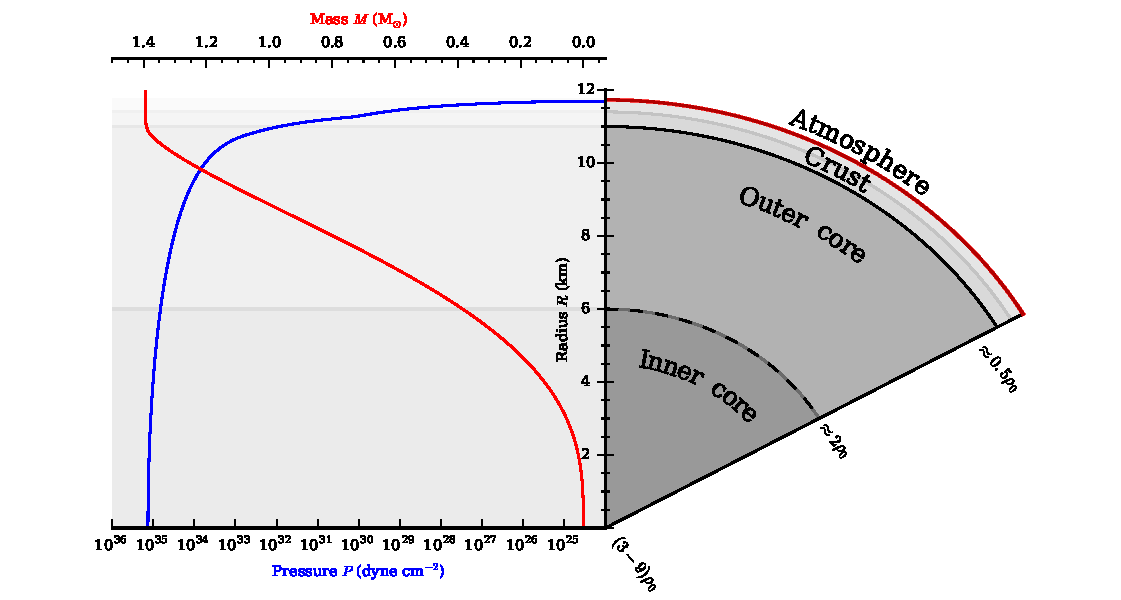
\includegraphics[width=13.5cm]{figs/slice/slice.pdf}
\caption{\label{fig:slice}
Overview of the neutron star structure for the SLy equation of state and core density of $P_{\mathrm{c}} = \Ten{8.9}{14}\gcm$, corresponding to $M=1.4\Msun$.
Right side of the figure shows a schematic presentation of the star's interiors against the radial coordinate, whereas the left side shows the pressure (blue; bottom axis) and cumulative mass (red; top axis) evolution from the core to the surface.
}
\end{figure}

\begin{figure}[t!]
\centering
\includegraphics[width=12cm]{figs/tov/core_eos.pdf}
\includegraphics[width=12cm]{figs/tov/mr.pdf}
\caption{\label{fig:coreMR}
Equation of states and the resulting neutron star mass-radius curves for the different core models.
\emph{Top:} Pressure versus density relation, $P(\rho)$.
\emph{Bottom:} Corresponding $M-R$ relations.
Symbols and colors are the same as in \fig{fig:coreGamma}.
}
\end{figure}

Instead of looking at the different quantities, such as the pressure, as a function of the density, let us now finally solve the structure of the star given the derived equations of states.
The results are obtained by numerically solving the Tolman-Oppenheimer-Volkoff equations using the previously presented crust model and the different equations of states for the core.%
\footnote{TOV-solver that is used is available from \url{https://github.com/natj/tov}.}
In \fig{fig:slice} the dependency of the pressure and cumulative mass of the star against the radial coordinate (as measured starting from the core) is visualized for the SLy equation of state for a central density of $P_{\mathrm{c}} = \Ten{8.9}{14}\gcm$, corresponding to $M=1.4\Msun$.
This visualizes the real dimensions of the neutron stars internal structure:
Inner core spans about $6\km$ in radius from the center while the outer core extends from $6$ to $11\km$.
The full crust is only about $\osim 1\km$ thick, and the atmosphere is too thin to be even visible.
The core also contains more than $99\%$ of the total mass of the star.



Instead of fixed central pressure, we can let it span a large range, starting from some small value and ending to the pressure corresponding to the maximum mass, to obtain mass$-$radius, or more succinctly, $M-R$ curves for the equations of states.
These are visualized in \fig{fig:coreMR} along with the pressure$-$density relations that yield them.
From here it is obvious how the large uncertainty in the nuclear physics of the core then translates into a large possible allowed radius range, from about $10$ to $15\km$.
It also opens up a pathway of probing the nuclear physics with astrophysics because  mass and radius measurements of real neutron stars can set constraints on the equation of state.


